%!TEX root = Main.tex


\section{Method}




	\subsection{k-means objective function}
		In what follows, we review the k-means objective function in the Euclidean space, and introduce the objective function in our case where the samples are realizations of point processes.

		% We will introduce the objective function of k-means in the Euclidean space as well as in our case where the samples are realizations of point process.
		\subsubsection*{k-means in $\mathbb{R}^d$} 
			Let ${\mathbf{x}_1,\cdots,\mathbf{x}_n}\in \mathbb{R}^d$ be an i.i.d. sample from distribution function $F$. Denote by $F_n$ the empirical distribution function. The k-means problem is to solve  
			\begin{align*}
			A_n:=\underset{A:A\subset \mathbb{R}^d, |A|=k}{\arg\min} W_n(A,F_n)=\underset{A:A\subset \mathbb{R}^d, |A|=k}{\arg\min}\int \min_{a\in A}\|\mathbf{x}_i-a\|^2  \text{d}F_n.
			\end{align*}

			There are some theoretical guarantees of k-means.
			\citet{Pollard1981a} shows that for a given $k$, $A_n\to \bar A $ almost surely, where $\bar A=\arg\min_A W(A,F) $ denotes the optimal population cluster centers.
			\citet{Bachem2017} provides a uniform bound with a rate of $\mathcal{O}\left(n^{-1/2}\right)$ for the deviation between the empirical loss and the expected loss. 
			The bound is uniform in the sense that it holds for any set of $k$ cluster centers.
			% \begin{align*}
			% \sup_{A}\big|W_n(A,F_n)-W(A,F)\big|= \mathcal O(n^{-\frac{1}{2}})
			% \end{align*}
			
			
			Note that $\bar A$ is a biased estimator of the true cluster centers (when they are well-defined).
			% {\color{red} What does $\bar A$ represent? 
			For example, if $k=2$ and $F(x)=\frac{1}{2}\Phi(x;\mu_1,\sigma_1^2)+\frac{1}{2}\Phi(x;\mu_2, \sigma_2^2)$ is a mixture Gaussian distribution, 
			and denote $X_1\sim N(\mu_1,\sigma_1^2)$, then $\bar A= \left\{ a_1,a_2 \right\} $ where $a_1=\mathbb{E}[X_1 \mathbf{1}_{X_1\leq (\mu_1+\mu_2)/2}]\neq \mu_1 $ (and a similar expression for $a_2$).

			
			This problem can be re-formulated as following 
			\begin{equation}\label{eq:kmeans}
			\min_{\left\{ \Gamma_l \right\}_{l=1}^k}\frac{1}{n}\sum_{l=1}^k\sum_{i\in {\Gamma}_l} \|\mathbf{x}_i- \mathbf{c}_l\|^2,
			\end{equation}
			where $\left\{ \Gamma_l \right\}_{l=1}^k$ represent the clusters and form a partition of $\Gamma = \left\{ \mathbf{x}_1,\mathbf{x}_2,\cdots,\mathbf{x}_n \right\}$,
			$\mathbf{c}_l = {1}/{|\Gamma_l|}\cdot\sum_{\mathbf{x}_i\in \Gamma_l}\mathbf{x}_i$ is the sample center of the $l$-th cluster. 
			For simplicity, we denote $\mathbf{x}_i\in \Gamma_l$ by $i\in\Gamma_l$ henceforth.
			{\color{red} The notation $\Gamma_l$ is introduced in 2.1 but for a different set of nodes. What is the appropriate way to re-define this notation?}
			We now extend this objective function to the context of point process.
		
		\subsubsection*{k-means in point processes}
			By Assumption \ref{asp:time lag} and \ref{asp:same distr}, 
			% $\lambda_{N_i}(t)=\lambda_{z_i}(t-\tau_i)+\sum_{l=1}^kf_{z_i,l}(t-\tau_i)\epsilon_{i,l}$, hence 
			$\lambda_{N_i}(t+\tau_i)\overset{d}{=}\lambda_{N_j}(t+\tau_j)$ for any $i,j$ satisfying $z_i=z_j$. Thus $F_{N_i}(t+\tau_i)\overset{d}{=}F_{N_j}(t+\tau_j)$ for any $i,j$ satisfying $z_i=z_j$, 
			where 
			$F_{N_i}(t):=\int_0^t\lambda_{N_i}(s)\text{d}s\big/\int_0^T\lambda_{N_i}(s)\text{d}s$.
			So the k-means problem is to solve
			% \begin{equation}\label{eq:kmeans_lambda}
			% \min_{\left\{ \Gamma_l \right\}_{l=1}^k} \frac{1}{n} \sum_{l=1}^k \left(\min_{\{\tau_i\}_{i\in\Gamma_l},\lambda_l} \sum_{i\in\Gamma_l} \|\hat\lambda_{N_i}(\cdot+\tau_i)- \lambda_l(\cdot)\|_2^2 \right),
			% \end{equation}
			% or, equivalently,
			\begin{align}\label{eq:kmeans_F}
			\min_{\left\{ \Gamma_l \right\}_{l=1}^k} \frac{1}{n} \sum_{l=1}^k \left(\min_{\{\tau_i\}_{i\in\Gamma_l},F_l} \sum_{i\in\Gamma_l} \| \tilde{F}_{N_i}(\cdot+\tau_i)- F_l(\cdot)\|_2^2 \right),
			\end{align}
			where 
			% $\hat \lambda_{N_i}(\cdot)$ is the intensity function estimated from $N_i(\cdot)$ using some smooth method,
			$\tilde{F}_{N_i}(t):=1/{N_i([0,T])}\cdot\sum_{j=1}^{N_i([0,T])}\mathbf{1}_{\{t_{N_i,j}\leq t\}}$ is the empirical distribution function of the occurrence time of edges,
			$t_{N_i,j}$ is the occurrence time of the $j$-th edge of $N_i(\cdot)$,
			and $F_l(t)=\mathbb{E}[F_{N_i}(t+\tau_i)] (\forall i\in\Gamma_l)$ is the expected cumulative distribution function of the $l$-th cluster.


			% Likelihood can also be used as a measure of similarity between a point process and an intensify function,
			% which yields the objective function
			% \begin{align}\label{eq:kmeans_likelihood}
			% \min_{\left\{ \Gamma_l \right\}_{l=1}^k} \frac{1}{n} \sum_{l=1}^k \left(\min_{\{\tau_i\}_{i\in\Gamma_l},\lambda_l} \sum_{i\in\Gamma_l} d\big({N_i}(\cdot+\tau_i), \lambda_l(\cdot)\big) \right),
			% \end{align}
			% where the distance is defined as the negative log-likelihood
			% \begin{align*}
			% d(N, \lambda) := -\log L(N;\lambda) = \int_{0}^T\lambda(t)\text{d}t - \sum_{j=1}^{N(0,T]}\log \left( \lambda(t_{N,j}) \right) .
			% \end{align*}
				
			% {\color{blue} Justify why it is reasonable to use Poisson process. }
			% % Also explain why this is a good measure of similarity.
	 		% {\color{blue} See \citet{Daley} for details.}

	 	% \subsubsection*{Other possible distance}
			% The squared error distance is defined as 
			% \begin{align*}
			% d(N,\lambda) := \int_0^T\lambda^2(t)\text{d} t - 2\int_0^T \lambda(t)\text{d}N(t)+?
			% \end{align*}



	\subsection{Algorithm}
		
		The initialization method and the choice of the number of clusters $k$ will be discussed later, now let us assume the initialization and $k$ are given.
		To solve the problem \eqref{eq:kmeans_F}, we iterate between two steps until convergence:
			\begin{itemize}
				\item Re-cluster step: update the clustering 
				$\left\{ \hat\Gamma_l \right\}_{l=1}^k$ based on the distance $d(\tilde{F}_{N_i}, \hat F_l)$ 
				defined as 
				\begin{align*}
				 d(\tilde{F}_{N_i}, \hat F_l) = \min\Big\{ \inf_{\tau\in[0,T]}\left( \int_{-T}^T\big| S_\tau\circ\tilde{F}^*_{N_i}(t)-\hat F_{l}^*(t) \big|^2 \text{d}t \right)^{1/2}, \\
				 \inf_{\tau\in[0,T]}\left( \int_{-T}^T\big| \tilde{F}^*_{N_i}(t)-S_\tau\circ\hat F_{l}^*(t) \big|^2 \text{d}t \right)^{1/2} \Big\},
				\end{align*}
				where
				\begin{align}\label{eq:def of shifted curve}
				S_\tau\circ\tilde{F}^*_{N_i}(t)=
				\begin{cases}
				0, &t\in[-T,-\tau)\\
				\tilde F_{N_i}(t+ \tau), &t\in[-\tau,T-\tau)\\
				1,& t\in [T-\tau,T]
				\end{cases},
				% \quad
				\hat F_{l}^*(t)=
				\begin{cases}
				0, &t\in[-T,0)\\
				\hat F_{l}(t), &t\in [0,T]
				\end{cases}.
				\end{align}
				
				
				\item Re-center step: update the expected cumulative distribution functions $\{\hat F_l\}_{l=1}^k$ using the method in \citet{Bigot2013}.

			\end{itemize}

		In the re-cluster step, the distance $d(\tilde F_{N_i}, \hat F_l)$ for each pair of node $i$ and cluster $l$ is evaluated by solving a (non-convex) optimization problem
		\begin{equation}
		\begin{aligned}\label{eq:aligned distance}
		\hat n_{i,l}&=\underset{n\in[0,N/2]}{\arg\min}\sum_{j=1}^{N-1}
		\left| \theta_{i,j}e^{\complexunit 2\pi j n/N}+
		\frac{e^{-\complexunit{}2\pi j}}{1-e^{\complexunit{}2\pi j /N}}\left( e^{\complexunit{}2\pi j n/N}-1 \right) 
		-\gamma_{l,j} \right|^2
		+ \left| \theta_0+n-\gamma_0 \right|^2
		\\
		&=\underset{n\in[0,N/2]}{\arg\min}\sum_{j=1}^{N-1}
		\left| \left( \theta_{i,j}+ \frac{e^{-\complexunit{}2\pi j}}{1-e^{\complexunit{}2\pi j /N}} \right) e^{\complexunit{}2\pi j n/N} 
		- \left( \gamma_{l,j}+\frac{e^{-\complexunit{}2\pi j}}{1-e^{\complexunit{}2\pi j /N}} \right)  \right|^2 
		+ \left| \theta_0+n-\gamma_0 \right|^2
		\\
		&\overset{\triangle}{=}\underset{n\in[0,N/2]}{\arg\min}\sum_{j=1}^{N-1}\left| \theta_{i,j}' e^{\complexunit{}2\pi j n/N} - {\gamma_{l,j}'}  \right|^2
		+ \left| \theta_0+n-\gamma_0 \right|^2
		,
		\end{aligned}
		\end{equation}
		where $n=N\cdot\tau/2T$,
		$\theta_{i,j}$ and $\gamma_{l,j}$,
		$j\in \mathbb{Z}$, are the discrete Fourier coefficients of $\tilde F^*_{N_i}$ and $\hat F^*_l$,
		$N$ is the length of discretized series of $\tilde F^*_{N_i}$ and $\hat F^*_l$.
		Grid search is used to solve problem \eqref{eq:aligned distance}.

		Gradient descent is not appropriate because the objective function oscillates rapidly and has too many local minima. 
		\begin{figure}[H]
		\centering
		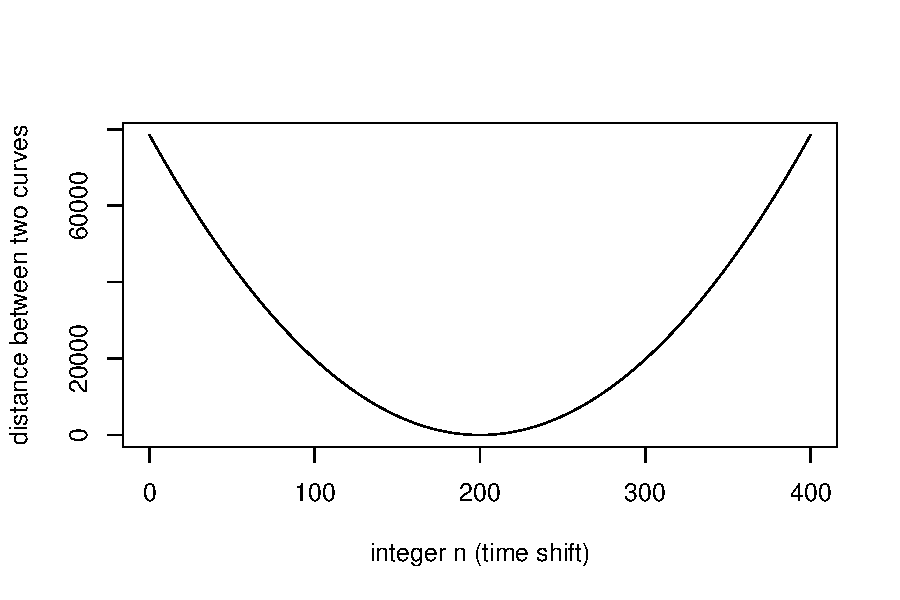
\includegraphics[width=0.7\textwidth]{../simulation/Dist_vs_integer_timeshift}\\
		\caption{The objective function is convex as a function of integer $n$.}
		\end{figure}
		\begin{figure}[H]
		\centering
		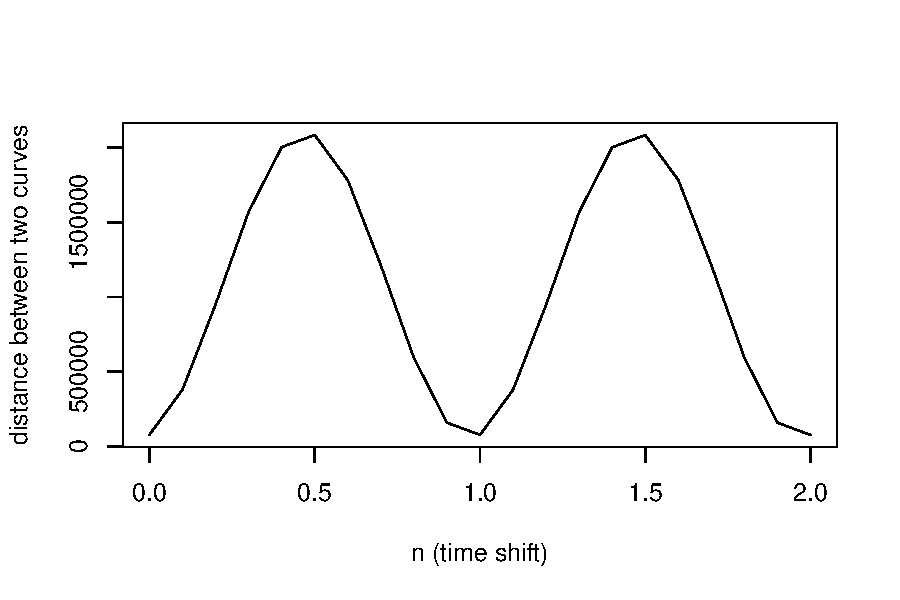
\includegraphics[width=0.7\textwidth]{../simulation/Oscillating}
		\caption{The function oscillates as a function of continuous $n$.}
		\end{figure}


		% Gradient:
		% \begin{equation}
		% \nabla = 4\pi \sum_{|j|\leq m} j\cdot \text{Im}\left( {\theta_{i,j}'}\overline{{\gamma_{i,j}'}}e^{\complexunit2\pi j\tau} \right) .
		% \end{equation}
		


		In the re-center step, let $\left\{ \theta_{i,j} \right\}_{j\in \mathbb{Z}}$ and $S_\tau\circ\tilde{F}^*_{N_i}(t)$ be defined the same as above.
		The Fourier coefficients of $S_\tau\circ\tilde{F}^*_{N_i}(t)$ are
		\begin{align*}
		\theta_{i,j}e^{\complexunit 2\pi j n/N}+
		\frac{e^{-\complexunit{}2\pi j}}{1-e^{\complexunit{}2\pi j /N}}
		\left( e^{\complexunit{}2\pi j n/N}-1 \right) 
		\overset{\triangle}{=}
		\theta_{i,j}' e^{\complexunit{}2\pi j n/N}-C. 
		\end{align*}
		Then
		$\left\{ \hat \tau_i \right\}_{i=1}^n = \left\{ \hat n_i\cdot 2T/N \right\}_{i=1}^n$ are obtained by 
		\begin{align*}
		\left\{ \hat n_i \right\}_{i\in\Gamma_l} &= 
		\underset{\min_{i\in\Gamma_l} \left\{ n_i \right\}=0}{\arg\min}
		\frac{1}{|\Gamma_l|}
		\sum_{i\in\Gamma_l}
		\sum_{j=1}^N 
		\left| 
		\theta_{i,j}' e^{\complexunit{}2\pi j n_i/N} -
		\frac{1}{|\Gamma_l|}\sum_{i'\in\Gamma_l}\theta_{i',j}' e^{\complexunit{}2\pi j n_{i'}/N}  
		\right|^2 
		.
		\end{align*}
		Again, gradient descent is not appropriate.
		Doing grid search over all $\left\{ n_i \right\}_{i\in\Gamma_l}$ is expensive, thus we adopt the following two-step estimation procedure:
		\begin{itemize}
			\item Estimate the mean distribution function $\hat F^*_l(t)$.
			\item Estimate $\left\{ \hat n_i \right\}_{i\in\Gamma_l}$ by aligning each $\tilde F^*_{N_i}(t) $ with $\hat F^*_l(t)$.
		\end{itemize}
		The initialization of $\hat F^*_l(t)$ can be any randomly chosen $\tilde F^*_{N_i}(t) $.

		% gradient:
		% \begin{align*}
		%  \frac{\partial L}{\partial \tau_i} = 
		%  \frac{1}{|\Gamma_l|^2}
		%  \sum_{|j|\leq m} 4\pi j
		%  \left( 
		%  	\text{Im}\left( \theta_{i,j}' e^{\complexunit{}2\pi j \tau_i}\cdot\overline{A_j}\right)+
		%  	\left(\frac{1}{|\Gamma_l|}-2\right) \text{Im}(A_j)\cdot 2 \text{Re}\left( \theta_{i,j}' e^{\complexunit{}2\pi j \tau_i}   \right) 
		%  \right) ,
		%  \end{align*}
		%  where $A_j=\frac{1}{|\Gamma_l|}\sum_{i\in\Gamma_l}\theta_{i,j}'e^{\complexunit{}2\pi j \tau_i} $.

		Finally, the mean distribution function is estimated as the average of shifted empirical distribution functions.		  



		\subsubsection*{Initialization}
			The initial mean curves are set to be randomly chosen empirical distribution function.

		\subsubsection*{Choosing $k$}
			



		% {\color{red} Should we take into account the error in $t_{N_i,j}$?}\\
		


		
		% Another direction is to use negative log-likelihood as the distance.
		% For reference see \cite{Vimond2010,Gamboa2007,Ronn2009,Gervini2005}.
		% The maximum likelihood estimator of the mean curve proposed in \citet{Gervini2005} is showed to be $\sqrt{n}$-consistent and asymptotically normal. % {(converge to a Gaussian process)}
		% {\color {red} But the log-likelihood includes unknown $f_{l,l'}$}
		% \begin{align*}
		% L(\lambda_{l},\tau_i;N_i)=\int \mathbb{P}\left( N_i(t)\Big| \lambda_{l}(t-\tau_i)+\sum_{l'=1}^k f_{l,l'}(t-\tau_i)\epsilon_{i,l'} \right) f(\epsilon_{i,1})\cdots f(\epsilon_{i,k})\\\text{d}\epsilon_{i,1}\cdots \text{d}\epsilon_{i,k}
		% \end{align*}
			


	\subsection{Convex relaxation of k-means type clustering}
		\subsubsection*{Semidefinite programming relaxation}
			We briefly introduce a semidefinite programming relaxation (Peng-Wei relaxation) of k-means proposed by \citet{Peng2005}.
			The k-means objective function in \eqref{eq:kmeans} can be re-written as
			\begin{align*}
			\sum_{l=1}^k\sum_{i\in\Gamma_l}\|\mathbf{x}_i- \mathbf{c}_l\|^2 &= \frac{1}{2}\sum_{l=1}^k \frac{1}{|\Gamma_l|}\sum_{i,j\in\Gamma_l}\|\mathbf{x}_i - \mathbf{x}_j\|^2\\
			&= \frac{1}{2}\sum_{l=1}^k\frac{1}{|\Gamma_l|}\langle \mathbf{1}_{\Gamma_l}\mathbf{1}_{\Gamma_l}^\top,\mathbf{D} \rangle
			\end{align*}
			where $\mathbf{D}\in \mathbb{R}^{n\times n}$ with entries $\mathbf{D}_{ij}=\|\mathbf{x}_i- \mathbf{x}_j\|^2$.
			\\
			Hence \eqref{eq:kmeans} can be relaxed to
			\begin{align*}
			&\min_{\mathbf{Z}}\ \langle \mathbf{Z},\mathbf{D}\rangle \qquad \\
			& \ \text{s.t. } \quad \mathbf{Z} \succeq 0, \quad \mathbf{Z} \geq 0, \quad \mathbf{Z} 1_{n}=\mathbf{1}_{n}, \quad \operatorname{Tr}(\mathbf{Z})=k.
			\end{align*}
		Proximity conditions are discussed in \ref{sec:proximity condition}.
		
		In our case, \eqref{eq:kmeans_lambda} is equivalent to 
			\begin{equation}\label{eq:unconvexified k-means}
			\min_{\mathbf{Z},\left\{ \tau_i \right\}_{i=1}^n}\langle \mathbf{Z}, \mathbf D(\tau_1,\cdots,\tau_n)  \rangle
			\end{equation}
		where $\mathbf{Z}=1/2\cdot \sum_{l=1}^k(1/|\Gamma_l|\cdot \mathbf{1}_{\Gamma_l}\mathbf{1}_{\Gamma_l}^\top)$, $\mathbf{D}_{i,j} = \| \hat\lambda_{N_i}(t+\tau_i)-\hat\lambda_{N_j}(t+\tau_j) \|_2^2$.
		Using Fourier transformation, 
		\begin{align*}
		\mathbf{D}_{i,j} &= \int_{0}^T \left( \int_0^\infty \hat h_{N_i}(\xi)e^{i2\pi\xi(t+\tau_i)}-\hat h_{N_j}(\xi)e^{i2\pi\xi(t+\tau_j)}\text{d}\xi \right)^2 \text{d}t
		\end{align*}
		where $\hat h_{N_i}(\xi)$ is the Fourier transform of $\hat\lambda_{N_i}(t)$. 
		% This seems not a convex function of $\tau_i$'s.
		{\color{red} How to convexify?}
		
		
		

	% \subsection{Other thoughts}
	% 	\begin{itemize}
	% 		\item What about using Fourier transformation and then k-means? What about functional principal component analysis?
	% 	\end{itemize}







